\chapterA{Hito 5 - Prototipado digital}

\section{Introducción}

Tras haber hecho en el hito anterior los primeros bocetos a papel para ver los
distintos escenarios de uso de la aplicación, ahora pasamos a un diseño digital que
representa mejor la visión final del producto. En esta sección recordaremos los puntos
más importantes del hito anterior.
\section{Factor de forma, postura y métodos de entrada}

Debido a que en el anterior hito estaban correctamente no hemos modificado nada, pero lo
incluimos en la memoria para mantener todos los apartados necesarios a la hora de hacer un prototipado.

Hemos creado los elementos de datos (transportes, billetes y viajes), junto con
sus atributos (por ejemplo, horario en el caso de transportes) y las relaciones
con otros elementos de datos, como los transportes y los viajes.

Posteriormente, se ha realizado la traducción de los requisitos funcionales en
elementos funcionales. De forma que describimos las acciones que podemos
realizar añadiendo una acción, un objeto y un contexto.

\subsection{Factor de forma}
Nuestra aplicación estará diseñada para móvil y ordenador. Si se utiliza desde
el ordenador, la aplicación se utilizará en mayoritariamente en casa para poder
organizar el viaje tranquilamente, aunque también puede utilizarse en un
contexto de trabajo en el que el usuario esté en una oficina. Si se utiliza la aplicación desde el
móvil el contexto cambia mucho, ya que normalmente el usuario hará un uso de la aplicación rápido para poder consultar información en cualquier parte o momento.

\subsection{Postura}
Por un lado tenemos varias \underline{posturas soberanas} centradas en toda la
parte de buscar destino, comparación de precios, ofertas o destinos a los que
acudir según las preferencias indicadas por el usuario. Por otro lado
tendríamos una \underline{postura temporal} relacionada con el chat de soporte
o con diferentes dudas que le puedan surgir al usuario que necesiten ser
subsanadas, así como diferentes reseñas que los usuarios hayan escrito sobre
los diferentes destinos. Por último tendríamos una \underline{postura demonio}
relacionada con las diferentes notificaciones que puedan surgir mediante el uso
de la aplicación (como la calificación o respuesta a una reseña hecha) y las
preferencias indicadas por el usuario.

\subsection{Métodos de entrada}
En caso de que se utilice la aplicación vía ordenador, los métodos de entrada
serán el teclado y ratón, mientras que si se accede a la aplicación por el
móvil, el método de entrada será la propia pantalla del teléfono.
\section{Elementos de datos}

En esta fase hemos definido los elementos de la interfaz que representarán los
requisitos identificados en la fase de identificación de requisitos.

Hemos creado los elementos de datos (transportes, billetes y viajes), junto con sus
atributos (por ejemplo, horario en el caso de transportes) y las relaciones con otros
elementos de datos, como los transportes y los viajes.

Posteriormente, se ha realizado la traducción de los requisitos funcionales en elementos
funcionales. De forma que describimos las acciones que podemos realizar añadiendo una acción,
un objeto y un contexto.

\subsection{Definición}

Tras un análisis de los errores cometidos en el hito anterior hemos definido los elementos
de la siguiente manera:

\begin{itemize}
    \item \textbf{Viaje}. Con este elemento representamos todos los datos sobre un desplazamiento
    concreto. Contará con los siguientes atributos:
    \begin{itemize}
        \item Fecha. Se marcará tanto el día de salida como el de llegada (pueden ser el mismo),
            con el formato en el orden correspondiente a la región (en España, \textit{dd/mm/aaaa}).
        \item Horario. La hora a la que sale el medio de transporte, además de la hora estimada de 
            llegada. El formato será \textit{HH:MM}, marcando la hora local del origen.
        \item Origen. Ciudad de la que sale el viaje, indicando la estación o aerpuerto correspondiente.
        \item Destino. Igual que con el origen, se guardará la ciudad de destino junto al lugar concreto.
        \item Accesibilidad. Si es un viaje accesible para personas con discapacidad o no.

    \end{itemize}

\end{itemize}

\section{Elementos funcionales}

Los elementos funcionales son las acciones que pueden ejercer los usuarios
sobre los datos que hemos definido en el apartado anterior. Los haremos basándonos
en los requisitos que hemos encontrados en los anteriores hitos.

Vamos a incluir todos los elementos funcionales, pero marcaremos aquellos que estén
repetidos con respecto al hito anterior.

\subsection*{Repetidos}

\begin{itemize}
    \item \textbf{Ofrecer \textit{(acción)} soporte al cliente \textit{(objeto)} para resolver problemas de gestión de
        billetes de manera rápida y eficaz. \textit{(contexto)}.}
        \begin{itemize}
            \item Desde cualquier pantalla se puede acceder a la pantalla de atención al cliente.
        \end{itemize}
\end{itemize}

\subsection*{Nuevos}

\begin{itemize}
    \item \textbf{Ofrecer \textit{(acción)} información detallada sobre las diferentes empresas que operan
        \textit{(objeto)} al comparar dos viajes \textit{(contexto)}.}
        \begin{itemize}
            \item Desde la página de \textit{Comparador} de viajes se puede hacer click en el logo de la empresa que
                opera para mostrar información e ir a la página del sitio.
        \end{itemize}
    
    \item \textbf{Ofrecer \textit{(acción)} información sobre las ayudas ofrecidas \textit{(objeto)} a usuarios 
        con discapacidad \textit{(contexto)}.}
        \begin{itemize}
            \item Desde la página de \textit{Comparador} se muestra la información sobre las ayudas a personas
                con discapacidad en el viaje.
        \end{itemize}

    \item \textbf{Buscar \textit{(acción)} transportes disponibles \textit{(objeto)} a las ciudades designadas \textit{(contexto)}.} 
        \begin{itemize}
            \item Desde la página \textit{Inicio} podemos seleccionar origen, destino y fechas en las que se quiera
                realizar el viaje.
        \end{itemize}

    \item \textbf{Filtrar \textit{(acción)} opciones de transporte \textit{(objeto)} específicas para personas con discapacidad
        física \textit{(contexto)}.}
        \begin{itemize}
            \item Desde la página \textit{Comparador} se pueden filtrar todas las opciones de transporte adecuadas para personas con
                discapacidad física.
        \end{itemize}
    
    \item \textbf{Reservar \textit{(acción)} billetes \textit{(objeto)} de los transportes deseados \textit{(contexto)}.} 
        \begin{itemize}
            \item Desde la página \textit{Comparador} se pueden seleccionar los billetes deseados y reservarlos.
            \item Desde la pantalla \textit{Datos adicionales de un viaje} se pueden seleccionar los billetes y reservarlos.
        \end{itemize}
    
    \item \textbf{Mostrar \textit{(acción)} información detallada \textit{(objeto)} sobre la accesibilidad de los transportes 
        disponibles \textit{(contexto)}.}
        \begin{itemize}
            \item Dentro de la información de cada transporte, se puede visualizar el nivel de accesibilidad del medio de
                transporte y seleccionar la ayuda si el usuario lo desea.
        \end{itemize}
    
    \item \textbf{Seleccionar \textit{(acción)} asientos \textit{(objeto)} una vez elegido el transporte \textit{(contexto)}.}
        \begin{itemize}
            \item Desde la pantalla \textit{Reserva} se pueden seleccionar los asientos deseados.
        \end{itemize}

    \item \textbf{Indicar \textit{(acción)} origen y destino \textit{(objeto)} del vehículo a lo largo del trayecto
        \textit{(contexto)}.}
        \begin{itemize}
            \item Desde la pantalla \textit{Reserva} se puede visualizar los detalles de la reserva del transporte, como el origen y el destino (tanto
                la ciudad como el lugar exacto).
            \item Desde la pantalla \textit{Comparador} se puede visualizar los detalles de la reserva del transporte, como el origen y el destino (tanto
            la ciudad como el lugar exacto).
        \end{itemize}
    
    \item \textbf{Ofrecer \textit{(acción)} asientos \textit{(objeto)} una vez elegido el transporte \textit{(contexto)}.}
        \begin{itemize}
            \item Desde la pantalla \textit{Reserva} se pueden seleccionar los asientos deseados.
        \end{itemize}

\end{itemize}
\section{Grupos funcionales y jerarquías}

En esta fase, una vez definidos los elementos de datos y funcionales, vamos a
organizarlos agrupándolos en unidades funcionales que nuestras personas el
trabajo en una tarea y la transición entre tareas. Para mostrarlo de manera más
visual hemos realizado un diagrama en árbol, para el que hemos usado el
programa \underline{\href{https://www.drawio.com/}{draw.io}}. Tras un análisis, 
hemos obtenido el resultado que observamos en la figura \ref{fig:jerarquias}, el cuál explicamos a 
continuación:
\begin{figure}[H]
      \centering
      \includegraphics[width=0.8\linewidth]{./Imagenes/jerarquia.png}
      \caption{Diagrama de jerarquías de funciones}
      \label{fig:jerarquias}
\end{figure}

\begin{itemize}
    \item La pantalla de inicio contiene los elementos de búsqueda, atención al cliente y mi perfil.
    \item El elemento de búsqueda es el componente principal por lo que ocupa gran espacio en la interfaz. Al usarla podrás realizar la selección de origen destino y/o fechas, así como de los viajeros. Estas opciones sirven como filtro a la hora de realizar la comparación, que se muestra a continuación.
    \item En el apartado de Comparador de viajes puedes ver todos los que cumplen los criterios anteriormente mencionados. Además puedes cambiar los filtros anteriores y/u ordenarlos según distintos criterios. Además podrás seleccionar si quieres que se muestren solo los viajes accesibles para personas con discapacidad física.
    \item Una vez te interesas por un viaje, pasarás al apartado de Reserva de transporte. Aquí se mostrarán todos los datos de manera clara, como se marcó en los requisitos, además de poder elegir los asientos y realizar la propia reserva del billete.
    \item En el apartado Mi perfil se puede cambiar los datos del usuario (nombre, correo, teléfono, etc) además de poder ver las reservas pasadas, pudiendo tanto cancelar el viaje como modificarlo (fecha u hora, siempre que lo permita la compañía).
    \item Como se comentó en el apartado anterior, se podrá acceder al apartado de atención al cliente desde cualquier punto de la aplicación.
    \item Un principio que podría ser útil para la aplicación es la programación orientada a objetos, debido a que tenemos distintas partes que podrían ser encapsuladas en éstos, como son los viajes.
    \item En cuanto a los patrones, uno de lo que podría usarse sería el patrón Singleton ya que asegura que cada clase tenga una única instancia, controla el acceso a cada recurso y tiene un control estricto de las variables disponibles.
\end{itemize}

\subsection{Orden general en que se usarán los elementos}

\begin{enumerate}

      \item Cambiar la configuración de idioma y moneda.
      \item Acceder a \textit{Atención al cliente} desde la \textit{Página principal}.
      \item Acceder a \textit{Perfil} desde la \textit{Página principal}.
      \item Funcionalidad principal: comparar distintas opciones de transportes según las
            necesidades.

\end{enumerate}

\subsection{Principios y patrones usados}

\begin{itemize}

      \item \textbf{Principio de proximidad.} Al agrupar elementos similares conseguimos que el usuario sepa que están relacionados, facilitando así el aprendizaje. Así como mejorar la memorabilidad, ya que el usuario puede relacionarlos mentalmente y recordarlos como grupo.
            Por ejemplo, la moneda y el idioma se han puesto cerca porque son dos elementos de configuración.
      \item \textbf{Principio de cierre.} Tendemos a buscar un único elemento simple.
            En nuestro caso, hemos puesto una barra deslizante para ver todo el contenido de la página.
      \item \textbf{Principio.} Los elementos de configuración, perfil y ayuda emplean los elementos de otros sistemas para que sea más fácil y rápido.
      \item \textbf{Principio de visibilidad y feedback.} La interfaz emplea distintos mecanismos para transmitir su estado actual y las acciones posibles en un determinado momento.
            Por ejemplo, en la pantalla de Comparador, pone los pasos que quedan para finalizar el proceso.
      \item \textbf{Ley de Von Restorff.} Destacar una funcionalidad por encima del resto.
            En la Página principal, queremos dar más importancia a la barra de búsqueda ya que es el objetivo principal de nuestra aplicación

\end{itemize}

\section{Prototipado}

Figma es una herramienta muy potente de diseño que permite la creación de prototipos
digitales altamente interactivos. Por ello, hemos empleado esta herramienta para poder
prototipar nuestras interfaces desarrolladas en el hito anterior, además de mejorarlas
aplicando aquellos cambios que se han considerado necesarios. Estos cambios serán explicados
en esta sección, además de detallar también los principios de diseño que aparecen en cada
una de las interfaces.

\subsection{Inicio}

La pantalla principal de nuestra aplicación (figura \ref{fig:it1_inicio}), como ya detallamos anteriormente, va a ser la de búsqueda,
en la que, a diferencia de lo planteado en el hito anterior, cualquier usuario va a poder realizar la
comparación de viajes (aunque no pueda finalizar sin tener que iniciar sesión o crearse una cuenta). Otro
de los cambios que además se ha realizado es ofrecer la posibilidad a los usuarios que no se hayan registrado
como discapacitados de poder buscar viajes accesibles sin tener que aplicar el filtro en la siguiente página
(el comparador). Sin embargo, a pesar de estos cambios, la esencia de la ventana es la misma, se mantiene la
barra de búsqueda con todas las opciones que se pedían anteriormente (el origen, el destino, la fecha de ida,
la fecha de vuelta y el número de asientos) y para completar se muestran las mejores ofertas en forma de
tarjetas para que el usuario vea de forma mucho más visual toda la información que ahí se expone. En cuanto a
los patrones y principios que se han seguido para esta pantalla, son los siguientes:

\begin{itemize}
    \item \textbf{Principio de proximidad.} Todos los campos requeridos para realizar una búsqueda se encuentran
        cercanos entre sí, además de encuadrados bajo un marco, lo que indica al usuario que todo el contenido
        solicitado es necesario para comenzar una búsqueda de transportes. Relacionado a ello, aplica la Ley de
        Fitts (la distancia que tiene que ser recorrida para moverse de un campo a otro es muy pequeña).
    \item \textbf{Consistencia interna.} Las distintas tarjetas que se presentan para mostrar las ofertas de la
        aplicación en la página de inicio guardan y muestran la misma cantidad de información: el logo de la compañía
        que lo opera, la fecha del viaje, el precio, las horas de salida y llegada y las estaciones. También presenta
        consistencia en cuanto a la forma de la tarjeta y los colores que se utilizan.
    \item \textbf{Consistencia externa.} Al igual que en la gran mayoría de las aplicaciones, cuando el usuario tiene la sesión
        iniciada en la página, puede acceder a su perfil pulsando sobre el botón de usuario situado en la esquina
        superior derecha.
    \item \textbf{Principio de visibilidad.} Del mismo modo que en el caso anterior, puede consultarse el estado en el que
        se encuentra la aplicación si en la esquina superior derecha te sale la opción de iniciar sesión o de
        registrarse (sesión no iniciada) o el icono del perfil (sesión iniciada).
\end{itemize}

\begin{figure}[H]
    \centering
    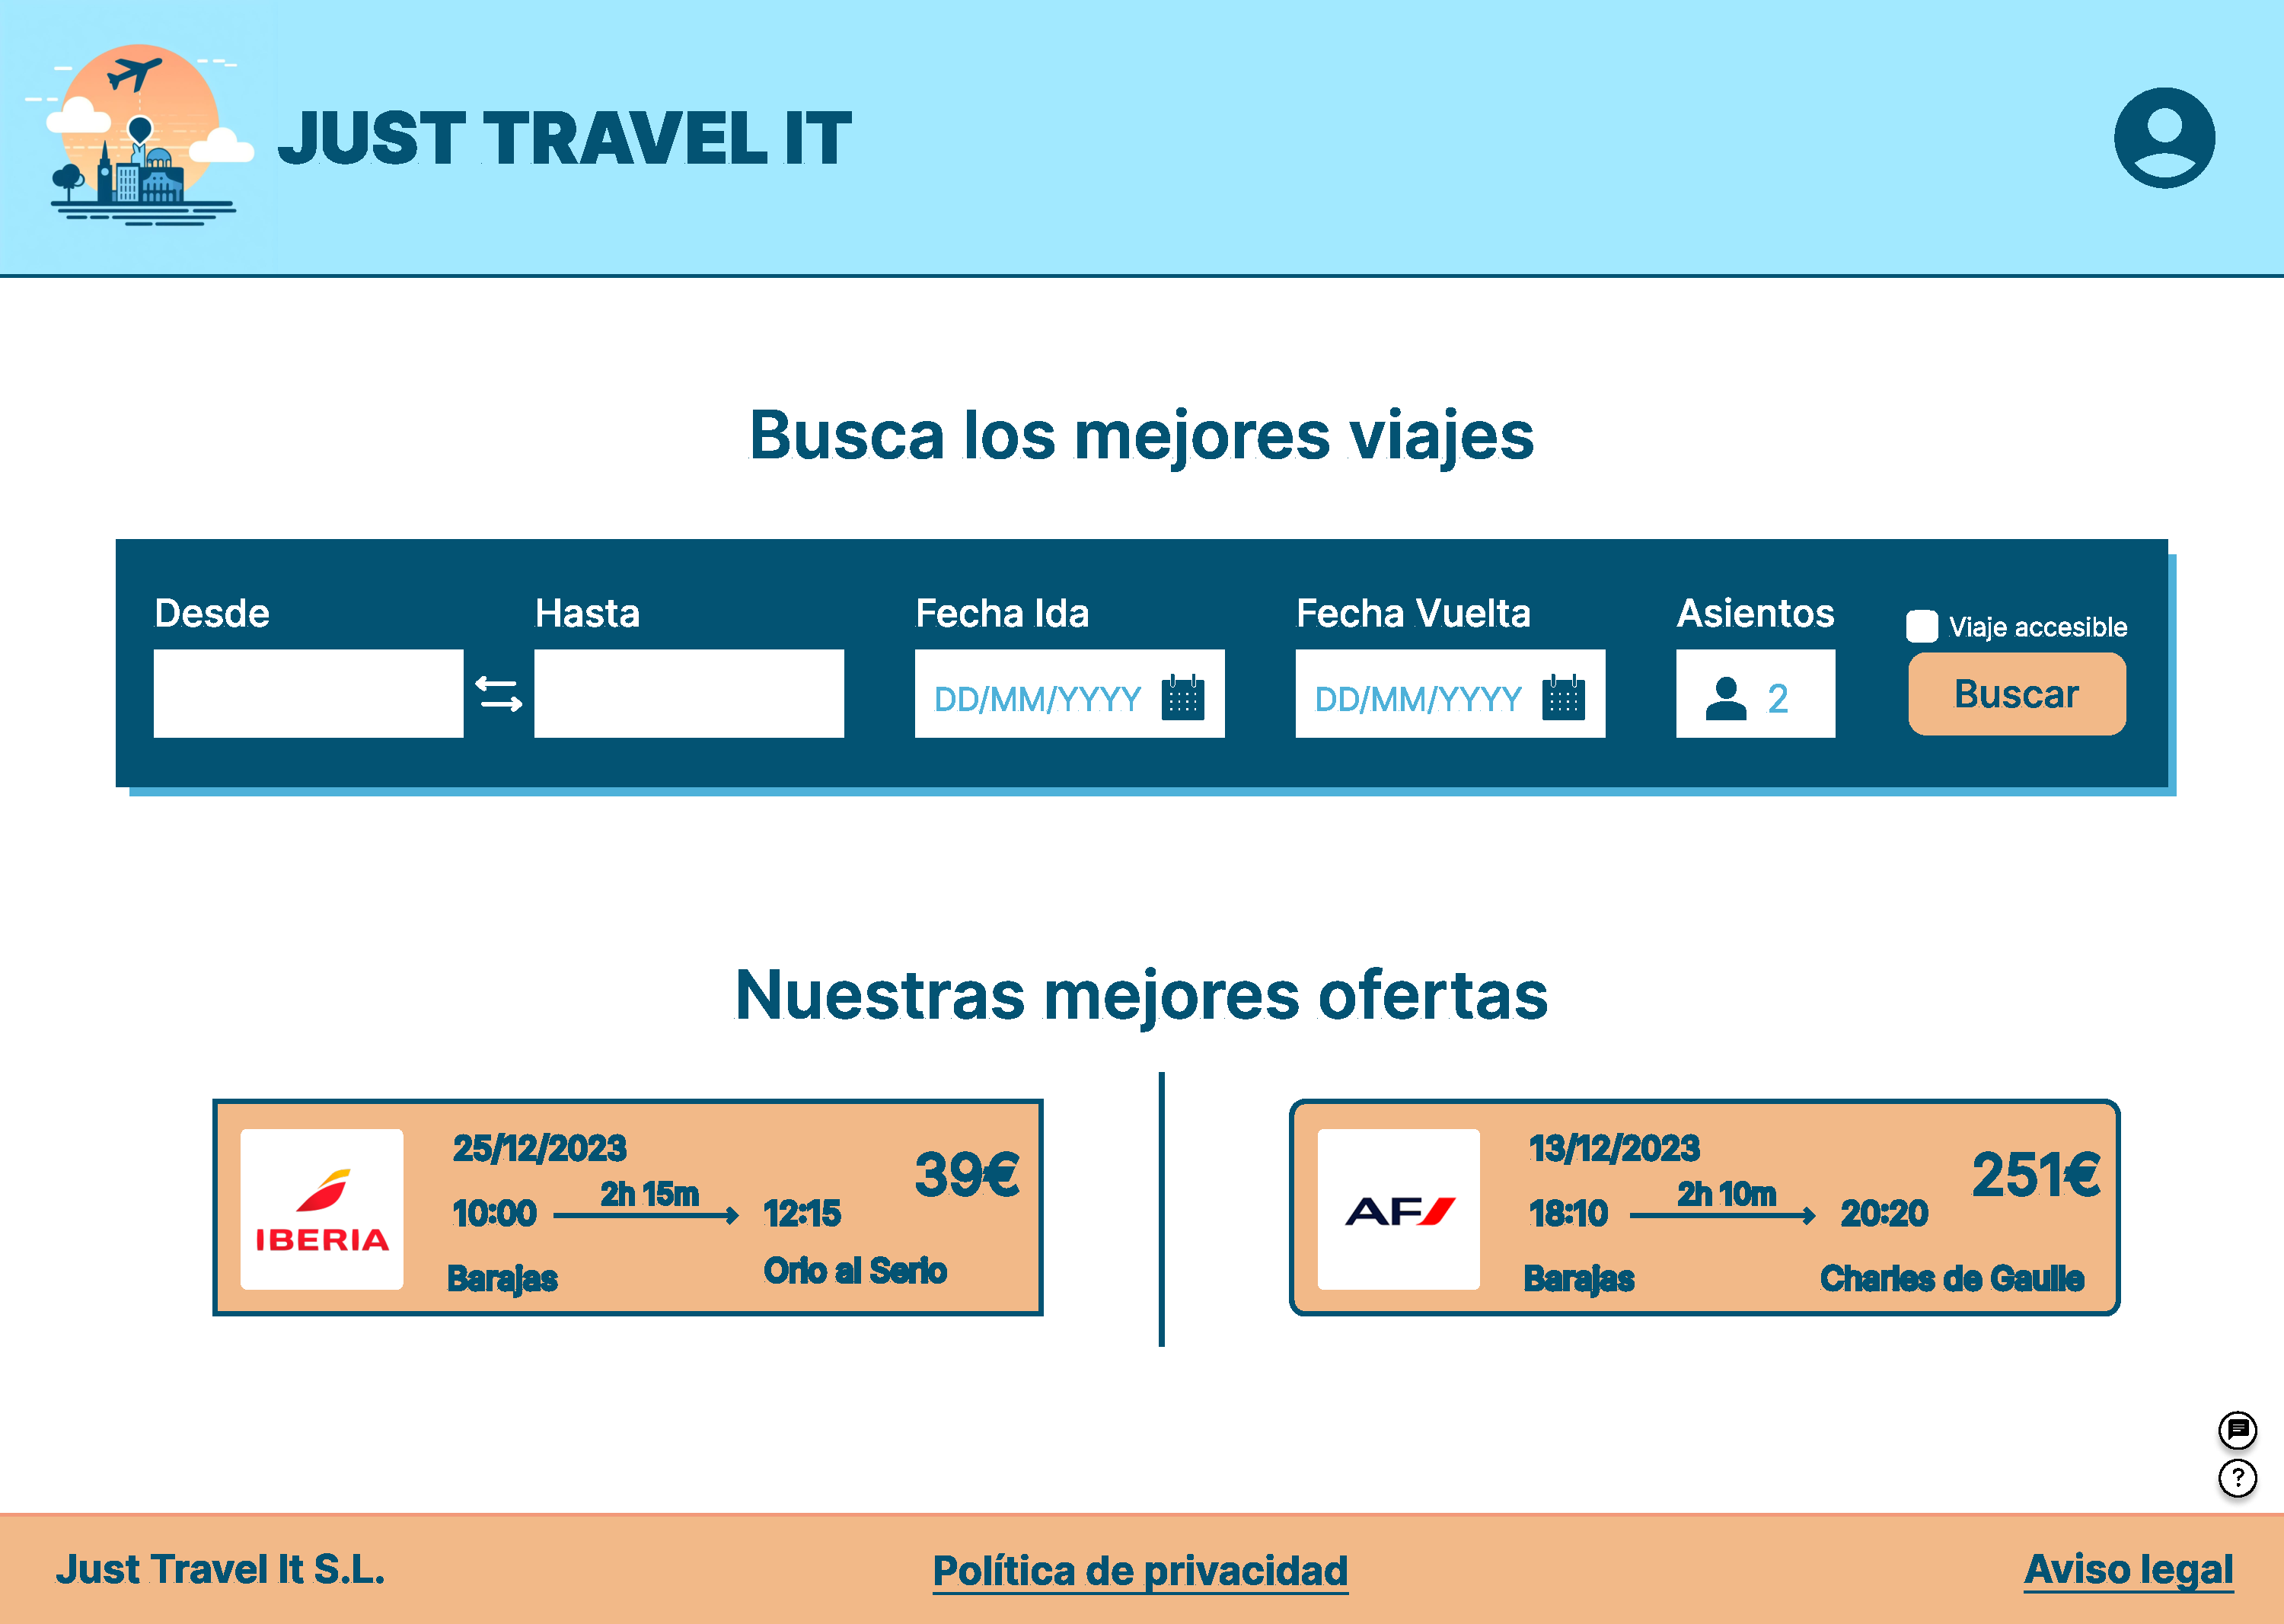
\includegraphics[page=1, width = 0.8\textwidth]{Imagenes/hito_5/it1.pdf}
    \caption{Página \textit{Inicio}}
    \label{fig:it1_inicio}
\end{figure}

\subsection{Comparador}

La pantalla del comparador (figura \ref{fig:it1_comparador}) no ha sufrido cambios con respecto al hito anterior, pero se ha cambiado el planteamiento
con respecto al hito anterior. Como ya hemos visto, dentro de la opción de búsqueda puedes seleccionar viajes
accesibles (aunque no seas una persona con discapacidad), apareciendo todos los viajes ya filtrados sin necesidad
de aplicar el filtro. Además, otra de las mejoras que se han realizado respecto a los prototipos en papel es hacer
que el botón de información de cada una de las tarjetas de los viajes muestre un \textit{pop-up} con la información más en
detalle del viaje: la información de las paradas que realiza (en caso de que las haya), la información del viaje
(la misma que se muestra en la tarjeta original), información de la compañía que opera el viaje (breve descripción
y un enlace a la página web), así como también los servicios adicionales que se ofrecen en el viaje. Se ha añadido
la funcionalidad de la ordenación de los viajes. En cuanto al contenido anterior de esta pantalla no se han realizado
modificaciones puesto que se ha considerado que la información que ya se mostraba tanto en los viajes como en los
filtros a aplicar era la necesaria. Una vez comentado el contenido de esta pantalla y las modificaciones que han
sido efectuadas, vamos a centrarnos en la identificación de los distintos patrones y principios que se han seguido
en el diseño de esta interfaz:

\begin{itemize}
    \item \textbf{Principio de proximidad.} Todas las tarjetas de los viajes de ida se encuentran bastante próximas entre
        sí y separadas de las tarjetas de viajes de vuelta, que entre sí también se encuentran cercanas, lo que
        indica que pertenecen a dos grupos distintos y claramente diferenciados. Por otro lado y aislado a este caso,
        el principio de proximidad también se aplica en el caso de las opciones de filtrado, ya que se encuentran
        todas agrupadas y próximas en la columna izquierda de la pantalla.
    \item \textbf{Consistencia interna.} al igual que ocurría con las ofertas que aparecían en la página de inicio, todas
        las tarjetas de viajes tanto de ida como de vuelta tienen la misma consistencia, puesto que la información
        que muestran y la tipografía y los colores que se utilizan son los mismos en todas las tarjetas. Otro de los
        ejemplos de la consistencia podemos observarlo en los filtros. Como puede apreciarse, aquellos filtros que se
        refieren a rangos (como el rango horario, el rango de precios o la duración), tienen el mismo formato de
        presentación, una barra en la que puedes moverte para seleccionar el filtro y unas barras que indican la
        cantidad de viajes que existen con esos valores.
    \item \textbf{Consistencia externa.} Además de la ya mencionada ubicación del botón del perfil (en la parte
        superior derecha de la pantalla), otras de las opciones que aparecen en esta pantalla y que guardan
        consistencia con la gran mayoría de las aplicaciones son los botones de Atrás y Continuar, ya que aparecen
        respectivamente en la parte izquierda y en la derecha de la aplicación, indicando la sensación de avance
        (derecha) y retroceso (izquierda).
    \item \textbf{Principio de visibilidad.} Uno de los mecanismos que tiene esta pantalla para informarte del estado de la
        misma es destacar el borde de aquellos viajes (tanto de ida como de vuelta) que hayas seleccionado, pudiendo
        conocer rápidamente las opciones que has escogido.
    \item \textbf{Ley de Hick.} Con la finalidad de no realizar un proceso de compra demasiado complejo y lleno de información,
        hemos decidido dividir el proceso en tres etapas: una primera etapa de selección de los viajes deseados,
        una segunda de datos y servicios adicionales y una tercera en la que se muestra un resumen y se procede al
        pago del viaje.
    \item \textbf{Efecto Zeigarnik.} Aunque la idea de dividir el proceso en distintas etapas se trate de un resultado de la
        Ley de Hick para intentar que sea mucho menos tedioso, la idea de mostrar la etapa del proceso en la que te
        encuentras para saber los pasos necesarios para finalizar es resultado de la aplicación directa del Efecto
        Zeigarnik.
    \item \textbf{Principio de libertad y control del usuario.} El usuario en todo momento tiene el control de la aplicación
        y puede decidir cuándo avanzar y cuándo retroceder en todo momento si ha detectado que ha cometido un error
        o bien quiere explorar otras opciones.
\end{itemize}

\begin{figure}[H]
    \centering
    \includegraphics[page=10, width = 0.8\textwidth]{Imagenes/hito_5/it1.pdf}
    \caption{Página \textit{Comparador}}
    \label{fig:it1_comparador}
\end{figure}

\subsection{Datos adicionales}

Al finalizar el proceso de selección de los viajes que se quieren reservar, la siguiente pantalla (figura \ref{fig:it1_datos_adicionales}) que aparece es
la de datos adicionales, que incluye: los datos de los pasajeros, si se desean contratar servicios
adicionales (gratuitos o bien pagando un suplemento) y la selección de los asientos. En cuanto a las modificaciones
que se han realizado con respecto al hito anterior han sido principalmente una modificación de la opción de seleccionar
asiento, ya que la información representada no era muy clara y además no mostraba información más allá de los asientos
(sólo mostraba la información de los huecos libres, sin dar información de la ubicación - filas y columnas - ni si
tenía o no ventanilla). Es por ello que se ha planificado una mejora en la que ahora se muestra una leyenda de
colores en función del estado del asiento (hemos añadido además asientos que debido a su posición dentro del vehículo
suponen un incremento del precio, por lo que se van a destacar en otro color). En cuanto a los principios de diseño que
aparecen en esta pantalla, podemos destacar los siguientes:

\begin{itemize}
    \item \textbf{Principio de cierre}. Dentro de la opción de seleccionar los datos de los pasajeros, puede verse
        cómo el campo del teléfono se encuentra entrecortado, dando la sensación a los usuarios de que puede seguir
        bajando para poder rellenar más datos.
    \item \textbf{Consistencia interna.} Las dos pestañas que se tienen para poder seleccionar los asientos y los servicios
        adicionales tienen la misma forma y tipografía, dando a entender al usuario la información contenida en
        ellas está altamente relacionada y es necesaria para poder continuar con la reserva del viaje.
    \item \textbf{Consistencia externa.} Además de la ya mencionada ubicación del botón del perfil (en la parte superior
        derecha de la pantalla), otras de las opciones que aparecen en esta pantalla y que guardan consistencia
        con la gran mayoría de las aplicaciones son los botones de Atrás y Continuar, ya que aparecen respectivamente
        en la parte izquierda y en la derecha de la aplicación, indicando la sensación de avance (derecha) y retroceso
        (izquierda).
    \item \textbf{Ley de Hick.} Con el fin de no sobrecargar la pantalla de información, los datos adicionales que se necesitan
        para la reserva se han dividido en tres secciones, de las cuales dos de ellas son desplegables, haciendo que
        la cantidad de información que se solicita al usuario puede ser regulada por él en todo momento.
    \item \textbf{Efecto Zeigarnik.} La idea de mostrar la etapa del proceso en la que te encuentras para saber los pasos
        necesarios para finalizar es resultado de la aplicación directa del Efecto Zeigarnik.
    \item \textbf{Principio de libertad y control del usuario.} El usuario en todo momento tiene el control de la aplicación
        y puede decidir cuándo avanzar y cuándo retroceder en todo momento si ha detectado que ha cometido un error
        o bien quiere explorar otras opciones.
\end{itemize}

\begin{figure}[H]
    \centering
    \includegraphics[page=11, width = 0.8\textwidth]{Imagenes/hito_5/it1.pdf}
    \caption{Página \textit{Datos adicionales}}
    \label{fig:it1_datos_adicionales}
\end{figure}

\subsection{Pago}

La última de las pantallas (figura \ref{fig:it1_pago}) necesarias para implementar la funcionalidad de realizar una reserva es la página de
pago. Una de las modificaciones realizadas (que ya mencionamos un poco anteriormente) es que antes de llegar a
esta página, si no tienes la sesión todavía iniciada, te requiere de hacerlo para poder continuar (al hacerlo te
vuelve a dirigir aquí con los datos de la compra que has realizado). En cuanto a las modificaciones realizadas
sobre la propia página, hemos mantenido la idea original de mantener los mapas de ida y de vuelta (mostrando el
itinerario a seguir) y pestañas en las que se dan dos posibles opciones de pago (tarjeta o PayPal). También
aparece el precio total del viaje, con el precio de los billetes más los suplementos que se hayan seleccionado
(servicios adicionales o asientos más caros). Sin embargo, a esto se le ha añadido un resumen de los viajes que
finalmente han sido seleccionados. Este resumen contiene las tarjetas de los viajes tanto de ida como de vuelta
y para cada una de ellas muestra la fecha, el origen, el destino y las fechas de salida y llegada. Además, cuando
se selecciona la opción de ver la información del vuelo, abre un \textit{pop-up} en el que se puede ver la información del
vuelo más detallada (los pasajeros que van a viajar, los asientos, los servicios que tiene disponibles y el precio). 

Otra de las modificaciones que se ha realizado es la información que aparece luego de confirmar la compra. En este
caso, hemos pasado de un \textit{pop-up} sencillo a una ventana en la que se muestra en detalle todo el resumen de la compra
que se ha realizado (las paradas, los destinos, las fechas, los pasajeros que van a viajar, los pasajeros y los
servicios adicionales que se han incluido en la compra). El mensaje con el número de la reserva diciendo que se ha
realizado correctamente se mantiene en la parte superior. Bajo esta información se encuentra un botón que da la
opción de continuar explorando nuevas opciones (lleva a la página de inicio). 

En cuanto a los principios de diseño que se han identificado (en ambas páginas, tanto en la referente a los datos
del pago como a la de confirmación de la compra), podemos encontrar los siguientes:

\begin{itemize}
    \item \textbf{Ley de Fitts.} Una vez decidido el método de pago con el que se va a realizar la reserva, los campos
        necesarios para efectuar la compra para cada uno de los métodos de pago se encuentran próximos entre sí
        (además de dentro de la misma pestaña), para poder facilitar al usuario moverse entre los distintos campos.
    \item \textbf{Consistencia interna.} La tipografía y los colores usados en las distintas opciones de pago (tanto en las
        pestañas como en los campos) es la misma, al igual que ocurre en el resumen de la compra (las tarjetas que
        representan los viajes de ida y de vuelta tienen la misma estructura y contienen la misma información para
        dársela al usuario). Esto también es aplicable al resumen de la compra, ya que la cantidad de información
        que se brinda en el viaje de ida es la misma que en el caso del viaje de vuelta.
    \item \textbf{Consistencia externa.} Como ya hemos visto en las etapas anteriores del proceso de reserva, se
        guarda cierta consistencia con el resto de aplicaciones, en las que se sobreentiende que el botón de retroceso
        de la página se encuentra en la parte derecha, mientras que en el caso de el de continuar (en este caso el
        botón de pagar) se encuentra en la parte derecha de la pantalla, dando la sensación de progreso.
    \item \textbf{Ley de Hick.} El número de opciones de pago que se ofrecen se encuentran separadas por pestañas,
        de modo que el usuario no se sobrecarga con una gran cantidad de información y de opciones con las que se
        puede realizar el pago.
    \item \textbf{Efecto Zeigarnik.} La idea de mostrar la etapa del proceso en la que te encuentras para saber los
        pasos necesarios para finalizar es resultado de la aplicación directa del Efecto Zeigarnik.
    \item \textbf{Principio de libertad y control del usuario.} El usuario en todo momento tiene el control de la aplicación
        y puede decidir cuándo avanzar y cuándo retroceder en todo momento si ha detectado que ha cometido un error
        o bien quiere explorar otras opciones.
    \item \textbf{Regla \textit{peak-end}.} Cuando se finaliza el proceso de reserva de la aplicación (\textit{peak}), se muestra a modo
        de finalización del proceso y para confirmar que todo se ha realizado correctamente una nueva ventana con
        un resumen de la información que se ha reservado.
\end{itemize}

\begin{figure}[H]
    \centering
    \includegraphics[page=8, width = 0.8\textwidth]{Imagenes/hito_5/it1.pdf}
    \caption{Página \textit{Pago}}
    \label{fig:it1_pago}
\end{figure}

\subsection{Inicio de sesión}

Para poder realizar reservas nuevas en la aplicación, es necesario que se inicie sesión (figura \ref{fig:it1_inicio_sesion}) con
una cuenta válida y que se encuentre ya registrada en la aplicación. Para poder realizar una
reserva completa sí que es necesario realizar el inicio de sesión, aunque para buscar viajes
no es necesario, como ya hemos visto anteriormente. Con respecto al prototipo del hito anterior
no se han realizado modificaciones aparentes sobre esta página, ya que se ha considerado que
la información que se solicita al usuario es la necesaria. En cuanto a los principios de diseño
que se han seguido para la creación de esta ventana son los siguientes:

\begin{itemize}
    \item \textbf{Ley de Fitts.} Los campos que han de rellenarse para poder iniciar sesión en la
        aplicación (correo y contraseña) se encuentran próximos entre sí, facilitando al
        usuario en todo momento el desplazamiento de uno a otro, pudiendo aportar de forma
        sencilla la información que le es solicitada.
    \item \textbf{Consistencia interna.} La tipografía y la disposición empleada para destacar los campos
        del formulario es la misma tanto en el caso del correo como en el de la contraseña (en
        la parte superior del campo se encuentra un texto que describe lo que ha de escribirse
        en el formulario y luego puede apreciarse el campo propiamente dicho).
    \item \textbf{Consistencia externa.} La página de inicio de sesión guarda consistencia externa con
        el resto de páginas de este tipo de las otras aplicaciones, ya que los campos de inicio
        de sesión se encuentran en la parte superior de la ventana, al igual que inmediatamente
        debajo de ello se encuentra el botón de iniciar sesión (si ya has rellenado los campos).
        Justo debajo de iniciar sesión, en caso de que todavía no tengas una cuenta se da la
        opción de registrarse como un nuevo usuario de la aplicación. Este ejemplo de estructura
        puede verse en el inicio de sesión de \textit{Gmail}, entre otros.
    \item \textbf{Principio de visibilidad.} Como ya vimos anteriormente, uno de los estados que va a
        manejar nuestra aplicación es el hecho de si tienes la sesión iniciada actualmente o no.
        Para poder consultar esta información, se puede observar la esquina superior derecha. Si
        el icono que aparece es el perfil, la sesión se encuentra iniciada, mientras que en el
        caso contrario, se requerirá de que se inicie sesión.
\end{itemize}

\begin{figure}[H]
    \centering
    \includegraphics[page=5, width = 0.8\textwidth]{Imagenes/hito_5/it1.pdf}
    \caption{Página \textit{Inicio de sesión}}
    \label{fig:it1_inicio_sesion}
\end{figure}

\subsection{Registro}

En el supuesto caso de que el usuario que quiera entrar a nuestra aplicación desee entrar para
poder realizar una reserva y no tenga una cuenta creada todavía, es posible darle la opción de
crearse una cuenta. Dentro de este nuevo formulario (figura \ref{fig:it1_registro}), al usuario le serán solicitados una serie
de datos adicionales (no solamente el correo y la contraseña). Estos datos adicionales han
variado con respecto al hito anterior, ya que se ha añadido nueva información para poder ofrecer
más facilidades al usuario, como por ejemplo, que a la hora de reservar un viaje, si tiene la
sesión iniciada, en los datos de los pasajeros se rellenará automáticamente la información del
primero de ellos con los datos que ya se tienen del usuario que se ha registrado en la aplicación.
En cuanto a los patrones de diseño que se han utilizado, hemos podido identificar los siguientes:


\begin{itemize}
    \item \textbf{Principio de proximidad.} Todos los campos que se necesitan para poder crear una nueva
        cuenta en la aplicación se encuentran próximos entre sí, permitiendo al usuario realizar
        movimientos muy cortos para desplazarse entre los distintos campos del registro.
    \item \textbf{Consistencia interna.} El fondo empleado tanto para cada uno de los campos así
        como la tipografía empleada para esta pantalla es consistente, ya que se mantiene dando
        una sensación de unidad en todo el conjunto de los datos.
    \item \textbf{Principio de visibilidad.} Como ya vimos anteriormente, uno de los estados que va a
        manejar nuestra aplicación es el hecho de si tienes la sesión iniciada actualmente o no.
        Para poder consultar esta información, se puede observar la esquina superior derecha. Si
        el icono que aparece es el perfil, la sesión se encuentra iniciada, mientras que en el
        caso contrario, se requerirá de que se inicie sesión.
\end{itemize}

\begin{figure}[H]
    \centering
    \includegraphics[page=2, width = 0.8\textwidth]{Imagenes/hito_5/it1.pdf}
    \caption{Página \textit{Registro}}
    \label{fig:it1_registro}
\end{figure}

\subsection{Perfil}

El usuario puede entrar a su perfil y visualizar todos los datos que haya introducido en el
registro (figura \ref{fig:it1_perfil}). Un usuario no registrado en \textit{Just Travel It} no puede acceder a esta pantalla ya que
para ello es necesario como mínimo tener un perfil en la aplicación. El usuario tampoco podrá
acceder a la pantalla de perfil si no está con sus sesión iniciada, puede ocurrir que el usuario
esté registrado pero no tenga la sesión iniciada, para ello debe iniciar sesión. En cuanto a los
principios de diseño que aparecen en esta pantalla, se pueden resaltar los siguientes:

\begin{itemize}
    \item \textbf{Consistencia interna.} El color utilizado en los botones es el mismo al igual
        que la fuente y el tamaño de la letra. No solo entre los botones dentro de la pantalla
        sino con los del resto de la aplicación.
    \item \textbf{Ley de Fitts.} La información de cada tipo se mantiene agrupada en su grupo. Los
        datos personales están todos juntos en un párrafo, mientras que la información general
        en otro, de esta forma se le facilita al usuario el encontrar la información que desee
        más ágilmente.
    \item \textbf{Ley de Hick.} Se aprovecha la clasificación del tipo de información del cliente para no
        agrupar todo en un bloque. De esta manera, evitamos que el usuario no se sobrecargue de
        información.
    \item \textbf{Principio de libertad y control del usuario.} El usuario tiene el control de su
        información en todo momento, siempre que tenga la sesión iniciada. Con esta pantalla
        tenemos el objetivo de mostrarle al usuario toda la información que ha metido en la
        aplicación y con el botón de modificar su perfil le damos la posibilidad de cambiar su
        información cuando desee.
\end{itemize}

\begin{figure}[H]
    \centering
    \includegraphics[page=12, width = 0.8\textwidth]{Imagenes/hito_5/it1.pdf}
    \caption{Página \textit{Perfil}}
    \label{fig:it1_perfil}
\end{figure}

\subsection{Modificar perfil}

Al usuario se le brinda la posibilidad de cambiar los datos de su perfil creado en \textit{Just Travel It} (figura \ref{fig:it1_mod_datos}). Podrá
modificar todos los campos rellenados en la creación del perfil. Ocurrirá lo mismo que en el \textit{Registro},
al modificar los datos, cuando se realice una reserva con la sesión iniciada se rellenaran los campos del perfil
en los campos adecuados a la reserva. Los principios empleados para la creación de esta ventana son:

\begin{itemize}
    \item \textbf{Consistencia interna.} La pantalla guarda consistencia sobre todo con la pantalla de la página de registro,
        los colores, tamaños, fuentes y tipografías se encargan de mantener la consistencia interna de estas pantallas.
    \item \textbf{Consistencia externa.} Se trata de la misma consistencia que podemos encontrar en \textit{Registro}.
    \item \textbf{Principio de proximidad.} Al ser igual que en \textit{Registro}, todas las preguntas se encuentran
        bastante próximas entre sí.
    \item \textbf{Principio de libertad y control del usuario.} El usuario en todo momento puede modificar todos
        sus datos introducidos en la aplicación.
    \item \textbf{Ley de Fitts.} Los campos que han de rellenarse para modificar el perfil se encuentran próximos
        entre sí y caben en la pantalla, por lo que no hay que hacer \textit{scroll} con el ratón, de este forma
        el usuario puede viajar con facilidad de un campo a otro.
\end{itemize}

\begin{figure}[H]
    \centering
    \includegraphics[page=4, width = 0.8\textwidth]{Imagenes/hito_5/it1.pdf}
    \caption{Página \textit{Modificar perfil}}
    \label{fig:it1_mod_datos}
\end{figure}

\subsection{Mis reservas}

Se le ofrece al usuario con una sesión iniciada que pueda consultar la información de sus reservas (figura \ref{fig:it1_reservas})
activas así como de poder comprobar las reservas pasadas. En este punto es posible consultar, modificar o cancelar
una reserva. Pasamos a nombrar los principios utilizados en esta pantalla: 

\begin{itemize}
    \item \textbf{Consistencia externa.} Al igual que en la gran mayoría de las aplicaciones, cuando el usuario
        tiene la sesión iniciada en la página, puede acceder a su perfil pulsando sobre el botón de usuario situado
        en la esquina superior derecha.
    \item \textbf{Principio de libertad y control del usuario.} El usuario en todo momento tiene el control de la
        aplicación y puede decidir cuándo avanzar y cuándo retroceder en todo momento si ha detectado que ha
        cometido un error en cuanto a la página a donde quería acceder.
    \item \textbf{Principio de visibilidad.} Como ya vimos anteriormente, uno de los estados que va a manejar
        nuestra aplicación es el hecho de si tienes la sesión iniciada actualmente o no. Para poder consultar
        esta información, se puede observar la esquina superior derecha. Si el icono que aparece es el perfil,
        la sesión se encuentra iniciada, mientras que en el caso contrario, se requerirá de que se inicie sesión. Además,
        se reconoce rápidamente la asociación ida-vuelta de los viajes.
    \item \textbf{Principio de proximidad.} Todas las tarjetas de los viajes de ida se encuentran bastante próximas entre sí
        y separadas de las tarjetas de viajes de vuelta, que entre sí también se encuentran cercanas, lo que indica
        que pertenecen a dos grupos distintos y claramente diferenciados.
\end{itemize}

\begin{figure}[H]
    \centering
    \includegraphics[page=3, width = 0.8\textwidth]{Imagenes/hito_5/it1.pdf}
    \caption{Página \textit{Mis reservas}}
    \label{fig:it1_reservas}
\end{figure}

\subsection{Consultar reserva}

Al usuario se le da la posibilidad de consultar su reserva (figura \ref{fig:it1_consulta_reserva}). Desde esta pantalla puede ver el viaje de ida y el
de vuelta, donde aparecen las tarjetas de los respectivos viajes, con las fechas, los días, la duración, la compañía,
la cantidad de pasajeros y la información adicional de la reserva. También se puede ver el mapa donde aparece la
ruta seguida en el viaje. Debajo del mapa se pueden consultar los datos de los pasajeros. Pasamos a nombrar los
principios utilizados en esta pantalla:

\begin{itemize}
    \item \textbf{Consistencia externa.} Al igual que en la gran mayoría de las aplicaciones, cuando el usuario
        tiene la sesión iniciada en la página, puede acceder a su perfil pulsando sobre el botón de usuario situado
        en la esquina superior derecha.
    \item \textbf{Consistencia interna.} La pantalla guarda consistencia sobre todo con la pantalla de la página
        resumen pago, los colores, tamaños, fuentes y tipografías se encargan de mantener la consistencia interna
        de estas pantallas.
    \item \textbf{Principio de proximidad.} Todos los campos que se necesitan para poder consultar una reserva en
        la aplicación se encuentran próximos entre sí, permitiendo al usuario realizar movimientos muy cortos para
        desplazarse entre los distintos campos.
    \item \textbf{Principio de libertad y control del usuario.} El usuario en todo momento tiene el control de la
        aplicación y puede decidir cuándo avanzar y cuándo retroceder en todo momento si ha detectado que ha cometido
        un error en cuanto a la página a dónde quería acceder.
    \item \textbf{Principio de visibilidad.} En esta pantalla se reconoce rápidamente la asociación ida-vuelta de los
        viajes.
    \item \textbf{Ley de Hick.} Con el fin de no sobrecargar la pantalla, los datos adicionales que se necesitan para
        la reserva se han dividido en dos secciones, haciendo que la cantidad de información que se muestra al
        usuario pueda ser regulada por él en todo momento.
\end{itemize}

\begin{figure}[H]
    \centering
    \includegraphics[page=6, width = 0.8\textwidth]{Imagenes/hito_5/it1.pdf}
    \caption{Página \textit{Consultar reserva}}
    \label{fig:it1_consulta_reserva}
\end{figure}


\subsection{Modificar reserva}

Al usuario se le otorga la posibilidad de modificar las reservas que haya realizado en \textit{Just Travel It} (figura \ref{fig:it1_mod_reserva}). Podrá
modificar los datos del pasajero: nombre, apellidos, DNI y teléfono. Tendrá a su disposición dos menús desplegables,
uno para poder contratar servicios adicionales que no haya contratado con anterioridad y otro en el que podrá
modificar su asiento. Además cuenta con un boton de selección en la parte inferior izquierda para poder solicitar
asistencia en la estación correspondiente por si se olvido de marcarlo a la hora de realizar la reserva. Pasamos
a nombrar los principios utilizados en esta pantalla:

\begin{itemize}
    \item \textbf{Consistencia interna.} La pantalla guarda consistencia sobre todo con la pantalla de la página
        mis reservas, los colores, tamaños, fuentes y tipografías se encargan de mantener la consistencia interna de
        estas pantallas.
    \item \textbf{Consistencia externa.} Al igual que en la gran mayoría de las aplicaciones, cuando el usuario tiene
        la sesión iniciada en la página, puede acceder a su perfil pulsando sobre el botón de usuario situado en la
        esquina superior derecha.
    \item \textbf{Ley de Fitts.} Los campos que han de rellenarse para modificar el perfil se encuentran próximos
        entre sí y caben en la pantalla, por lo que no hay que hacer \textit{scroll} con el ratón, de este forma
        el usuario puede viajar con facilidad de un campo a otro.
    \item \textbf{Principio de libertad y control del usuario.} El usuario en todo momento tiene el control de la
        aplicación y puede decidir cuándo avanzar y cuándo retroceder en todo momento si ha detectado que ha cometido
        un error en cuanto a modificar los datos.
    \item \textbf{Principio de proximidad.} Todos los campos que se necesitan para poder modificar una reserva en
        la aplicación se encuentran próximos entre sí, permitiendo al usuario realizar movimientos muy cortos para
        desplazarse entre los distintos campos a modificar.
    \item \textbf{Principio de visibilidad.} Como ya vimos anteriormente, uno de los estados que va a manejar nuestra
        aplicación es el hecho de si tienes la sesión iniciada actualmente o no. Para poder consultar esta
        información, se puede observar la esquina superior derecha. Si el icono que aparece es el perfil, la sesión
        se encuentra iniciada, mientras que en el caso contrario, se requerirá de que se inicie sesión.
\end{itemize}

\begin{figure}[H]
    \centering
    \includegraphics[page=7, width = 0.8\textwidth]{Imagenes/hito_5/it1.pdf}
    \caption{Página \textit{Modificar reserva}}
    \label{fig:it1_mod_reserva}
\end{figure}

\subsection{Soporte}

Si un usuario tiene alguna pregunta que no pueda ser abordada mediante el apartado de preguntas frecuentes previamente
mencionado (figura \ref{fig:it1_soporte}), ya sea debido a la naturaleza altamente específica de su problema o porque requiere una solución no
automatizada, o si experimenta algún inconveniente con la aplicación, tiene la opción de hacer clic en el incluíacono de
chat. Este icono se encuentra ubicado en la parte inferior derecha de cualquier pantalla de la página web, justo sobre
el icono de preguntas frecuentes.

Esta pantalla ha experimentado ciertas modificaciones con respecto al prototipo en papel. En este caso, hemos
expandido las funcionalidades de la sección de soporte, que anteriormente sólo incluía un asistente automatizado
de respuestas. La nueva sección ahora incorpora un canal de contacto telefónico, donde los usuarios pueden obtener
toda la información necesaria para comunicarse con un asistente personal. Además, hemos añadido una función de
mensajería que permite a los usuarios enviar mensajes y solicitudes directamente al equipo de asistencia al cliente,
que responderá con la mayor brevedad posible.

En cuanto a los principios de diseño que se han seguido para la creación de estas ventanas, son los siguientes:

\begin{itemize}
    \item \textbf{Principio de proximidad.} Todos los campos que se necesitan rellenar para poder enviar un nuevo
        mensaje, se encuentran próximos entre sí, permitiendo al usuario realizar movimientos muy cortos para
        desplazarse entre los distintos cuadros de texto. Relacionado a este principio, aplica la Ley de Fitts,
        donde la distancia que tiene que ser recorrida para moverse de un campo a otro es muy pequeña.
    \item \textbf{Consistencia interna.} Las distintas tarjetas que representan las formas de contactar con atención
        al cliente, tienen la misma estructura: un icono significativo, el significado de la tarjeta e información
        añadida en caso de ser necesaria. También presenta consistencia en cuanto a la forma de la tarjeta y los
        colores que se utilizan.
    \item \textbf{Consistencia externa.} Se guarda cierta consistencia con el resto de aplicaciones. Icono de
        perfil, botón de atrás y enviar, en el chat; el botón de enviar y el cuadro de texto para escribir (simulando
        el mismo que encontraríamos en un teléfono), una “X” que indica “cerrar el \textit{pop-up}”.
    \item \textbf{Feedback visual.} Una vez enviada la solicitud o mensaje al equipo de asistencia al cliente, el
        usuario recibirá un mensaje de confirmación con el objetivo de aclarar las dudas de si el mensaje ha sido
        enviado con éxito.
    \item \textbf{Principio de libertad y control del usuario.} El usuario mantiene el control total de la aplicación,
        teniendo la capacidad de avanzar o retroceder en cualquier instante. Si identifica un error o desea
        explorar alternativas, cuenta con la libertad de tomar decisiones de manera autónoma en todo momento.

\end{itemize}

\begin{figure}[H]
    \centering
    \includegraphics[page=13, width = 0.8\textwidth]{Imagenes/hito_5/it1.pdf}
    \caption{Página \textit{Soporte}}
    \label{fig:it1_soporte}
\end{figure}

\subsection{Preguntas frecuentes}

Si un usuario quiere consultar las preguntas frecuentes que pueden surgir a la hora de utilizar la aplicación,
es posible darle al botón de preguntas frecuentes marcado con una interrogación en la parte inferior derecha
de la pantalla. Esta pantalla (figura \ref{fig:it1_faq}) con respecto al prototipo en papel no ha tenido ningún cambio. Pasamos a nombrar
los principios utilizados en esta pantalla:

\begin{itemize}
    \item \textbf{Consistencia interna.} La tipografía y los colores usados en las distintas preguntas frecuentes
        es la misma, al igual que ocurre en las preguntas frecuentes desplegables. 
    \item \textbf{Consistencia externa.} Se guarda cierta consistencia con el resto de aplicaciones, empleando el
        desplegable en las preguntas para después mostrar las preguntas frecuentes relacionadas.
    \item \textbf{Principio de proximidad.} Todas las preguntas se encuentran bastante próximas entre sí.
    \item \textbf{Principio de libertad y control del usuario.} El usuario en todo momento tiene el control de la
        aplicación y puede decidir cuándo avanzar y cuándo retroceder en todo momento si ha detectado que ha cometido
        un error entrando en la pregunta que no debía o bien quiere explorar otras preguntas.
    \item \textbf{Ley de Fitts.} Los campos que han de rellenarse para modificar el perfil se encuentran próximos
        entre sí y caben en la pantalla, por lo que no hay que hacer \textit{scroll} con el ratón, de este forma el
        usuario puede viajar con facilidad de un campo a otro.
\end{itemize}

\begin{figure}[H]
    \centering
    \includegraphics[page=9, width = 0.8\textwidth]{Imagenes/hito_5/it1.pdf}
    \caption{Página \textit{Preguntas frecuentes}}
    \label{fig:it1_faq}
\end{figure}

\section{Escenarios keypath}

Los escenarios keypath son una evolución de los escenarios de contexto que describen detalladamente la interacción entre el usuario y el producto, una técnica de modelado que consiste en describir de manera narrativa cómo utiliza el usuario el producto para lograr sus objetivos. Estos escenarios muestran de manera detallada las funcionalidades del sistema y cómo interactúa el usuario con él.

\subsection{Escenario 1 - Marta}

``Marta quiere ir a las distintas ciudades del norte de Italia de la gira de Francesca, por lo que abre en el ordenador la aplicación e inicia sesión, para en la página de inicio de la aplicación hace clic al icono de usuario y como no está registrada le muestra la pantalla de inicio de sesión, introduce el correo electrónico y su contraseña y le da al botón de iniciar sesión y le redirige a la página de inicio con sesión iniciada.''

``Una vez iniciada la sesión y en la página de inicio, en el buscador selecciona como origen Madrid, como destino la primera ciudad de la gira y las fechas, con el calendario de la página tanto haciendo clic en el calendario de fecha de ida y de vuelta, que habían planificado quedarse en esa ciudad para luego ir a la próxima ciudad según la ruta diseñada y selecciona dos viajeros, ya que va a ir con su hermano y por selecciona un joven y un adulto.''

``Para el primer viaje ha tenido que filtrar los resultados en avión marcando el botón vuelos, ya que tienen que viajar de un país a otro para la primera ciudad y lo más rápido posible. Los resultados aparecen ordenados como predeterminados por fechas, así que no toca la opción de ordenar. Como no tiene ninguna preferencia en filtros no toca la parte izquierda de la página y empieza a navegar primero por los resultados de ida (en la parte izquierda) y selecciona el que le parece mejor y hace lo mismo que los resultados de la vuelta (en la parte derecha) y lo selecciona. Una vez seleccionados ambos viajes le da clic al botón de siguiente.''

``En el siguiente paso, que es la ventana de reserva, Marta rellena sus datos, es decir, pone su nombre, apellidos, DNI, teléfono y correo electrónico en sus campos correspondientes, También selecciona los asientos de ida y vuelta desplegando sus correspondientes menú, siempre elige un asiento asegurándose de que haya al menos un asiento libre para su hermano. Una vez que ha terminado, le da clic al botón de siguiente para hacer lo mismo su hermano. Cuando su hermano ha terminado de rellenar la al botón de siguiente, que le redirige al pago de los billetes.''

``En la página de pago comprueban los asientos mediante haciendo clic en detalles de cada resumen de cada billete y ven que todo está bien. Una vez comprobado esto despliega el menú de tarjeta de crédito y pone el número de la tarjeta, la fecha de caducidad, el nombre del titular y el CVC. Una vez introducida toda la información, presiona pagar y se redirige a la ventana de resumen de pago.''

``En la ventana de resumen de pago miran los dos billetes bien (el de ida y el de vuelta), es decir, comprueban los aeropuertos, el mapa, que la información de los pasajeros estén bien y los asientos estén bien y los descargan y finalmente le dan a seguir explorando porque tienen que comprar más billetes del resto de ciudades del tour.''

Video: ``Marta compra billetes de la primera ciudad del tour''\footnote{Video 1: \url{https://drive.google.com/file/d/1Cyn-CuykGe-TGzzBjvQFO50h13yFxktR/view?usp=drive_link}}.

``Para el resto de ciudades, hace el mismo procedimiento, a excepción de no poner filtro de medio de transporte en los resultados de la página del comparador, ya que en esos casos da igual mientras cumpla con lo planeado. También cambia que en la ventana de reserva tenga que mirar los servicios adicionales de algunos viajes para contratar el servicio de comida y cama. Por el resto es exactamente igual.''

Video: ``Marta selecciona servicios''\footnote{Video 2: \url{https://drive.google.com/file/d/15AvnvEH5TOCA40rL0Bms_vTr6Ml_wfH8/view?usp=drive_link}}.

``Marta ha tenido que volver a meterse en su perfil a través del icono de usuario en la página de inicio de la aplicación para cancelar un viaje ya que la cantante ha cancelado el concierto en esa ciudad. Para ello le ha dado a la botón con una cruz a la derecha del viaje que quería cancelar y le ha salido un ventana emergente y finalmente ha podido cancelar.''

Video: ``Marta cancela viaje''\footnote{Video 3: \url{https://drive.google.com/file/d/13Jwa1nbN0I86aLVI_jAmkjUNPgPpaHe8/view?usp=drive_link}}.

``Debido a este último cambio, Marta ha tenido que ver si puede adelantar la fecha de ida y cambiar el lugar de origen de la siguiente ciudad a través de comprar un nuevo billete y como si había, compra de la misma forma que antes dos billetes (para su hermano también) con la nueva fecha de ida y cancela el que tenía antes comprado de la misma forma. Como solo quedaban dos asientos ha tenido que rellenar muy rápido los datos en la página de reserva y una vez que ha terminado de pagar, ha empezado a dudar de si había puesto bien los datos. Por lo que desde la página de inicio hace clic en su foto de perfil y le redirige a la ventana de perfil. Ahí hace clic en el botón de mis reservas y ve su lista de reservas. Navega por la página hasta encontrar ese viaje y le da al botón de ver (en forma de ojo) y al comprobar los billetes, efectivamente ha puesto su número y DNI mal. Así que vuelve atrás con el botón de volver y hace clic en el botón de modificar (con el icono de un lápiz) y va al campo de teléfono y dni y lo modifica y le da a confirmar cambios. Y ya está listo su viaje.''

Video: ``Marta modifica sus datos''\footnote{Video 4: \url{https://drive.google.com/file/d/1T5jODli8WcZ8USFsLWabHf4M-UU_7SjH/view?usp=drive_link}}.


\subsection{Escenario 2 - Marta}

``Como dentro de poco son los exámenes y Marta está agobiada, su amiga Pili le ha sugerido ir a Ibiza el fin de semana posterior a los exámenes para relajarse. A Marta le ha parecido bien la idea así que coge su portátil y abre la aplicación con la sesión ya iniciada y en la sección de búsqueda escribe como origen Madrid y como destino Ibiza. Para las fechas las escribe de forma manual en vez de usar el calendario interactivo que son los días del fin de semana acordado. Pone el número de pasajeros a 2 jóvenes y le da al botón de buscar y le redirige a la página de comparador.
Una vez en la página del comparador empieza ordenando los resultados mediante el botón de ordenar y escoger la opción de ordenar por precio de forma creciente pero ve que no son precios muy asequibles, así que aplica el filtro de precio a 50 euros máximo en la parte izquierda y ahora no hay ningún resultado.''

Video: ``Marta filtra resultados''\footnote{Video 5: \url{https://drive.google.com/file/d/1o30b25FNA6LnXUABWE4MGlyzKMH3CAdA/view?usp=drive_link}}.

``Como no podía subir más su presupuesto, vuelve al inicio de la página con el botón de atrás mientras piensa y ve las ofertas que hay al principio y ve que ir a Palma de Mallorca sale 20 euros la ida y vuelta cada uno. Así que después de que Pili cediera al cambio de planes, selecciona en el buscador como origen Madrid, destino Palma de Mallorca, las mismas fechas (igual que antes) y los mismos asientos (2 jóvenes) y pone el filtro de 20€ para que aparezcan antes esos billetes y efectivamente aparecen.''

Video: ``Marta se fija en las ofertas''\footnote{Video 6: \url{https://drive.google.com/file/d/1NEVMNbseElLRKjDC75WIpdf4-KpuRgj-/view?usp=drive_link}}.

``La compra de los billetes es igual que en el primer escenario de Isabel.''


\subsection{Escenario 1 - Isabel}

``Mientras espera el desayuno, Isabel recibe una llamada de su jefe informando sobre la conferencia para la inclusión de niños con discapacidad y la necesidad de encontrar un sustituto para la potente original. Debido a la urgencia, Isabel acepta la propuesta y decide ponerse a buscar transporte para asistir a la conferencia.''

De esta forma, enciende el portátil y busca la aplicación. Una vez abierta, debido a que no tiene una cuenta, decide crearla con la intención de simplificar el proceso para las próximas veces. Para ello, en la página inicial selecciona ``crear cuenta'', lo que la desplaza a una nueva pantalla de registro en la que rellena todos los datos requeridos, nombre, apellidos, fecha de nacimiento, nacionalidad, teléfono, contraseña, entre otros.

Una vez creada su cuenta, se inicia sesión automáticamente y vuelve a la pantalla principal.
Es en esta pantalla donde introduce los datos relativos a su búsqueda de viaje. En el buscador selecciona como origen Barcelona, como destino Madrid, fecha de ida el día actual y fecha de vuelta el miércoles(día en el que tiene la conferencia). Además indica el número de asientos a 1 adulto y marca la casilla de ``viaje accesible''(debido a su condición física) y pulsa en el botón de ``Buscar'' para acceder al comparador.  

Debido a la casilla de ``viaje accesible'' marcada en el buscador, se le despliega la variante del comparador de viajes dedicada a su condición física lo que le permite visualizar de forma más ágil los transportes adecuados. Como el motivo de viaje es urgente, en la sección tipo de transporte selecciona ``vuelos'', para visualizar únicamente los vuelos que cumplan sus condiciones. Además hace uso de los filtros del lateral izquierdo, selecciona viaje directo para evitar transbordos, establece un margen de precio no superior a unos 200 euros y pulsa en el botón ``filtrar'', lo que actualiza la lista de billetes adecuados. Por último utiliza la ordenación por precio inferior en la casilla en la parte superior derecha.

Ya con las opciones disponibles delante, selecciona el billete de ida y vuelta que más le convence y pulsa el botón ``siguiente'' que la lleva al siguiente paso.

En este paso que corresponde a la ventana de reserva Isabel rellena sus datos, nombre, apellidos, DNI, teléfono, etc. Además pulsando en los desplegables, selecciona los asientos de ida y de vuelta disponibles que más le agrade teniendo en cuenta sus limitaciones. Una vez seleccionados los asientos pulsa en ``siguiente'', comenzando así el último paso correspondiente al pago del billete..


En la página de pago comprueba los detalles del billete y selecciona la opción pagar con tarjeta de crédito, introduciendo todos los datos necesarios, número de tarjeta,fecha, titular, cvc, y presiona el botón ``pagar'' para realizar el pago. Es entonces cuando se actualiza la página mostrando un resumen de la compra.

Ya con el billete en su correo, Isabel se siente satisfecha con la utilidad y simplicidad de la aplicación, se dirige a su perfil  para cerrar sesión pulsando en ``cerrar sesión'' y aceptando la confirmación y se dirige a casa a preparar su maleta.

Video: ``Escenario 1 Isabel''\footnote{Video 7: \url{https://drive.google.com/file/d/1zxenSnsUoDwXNdjQV03FPnIg7N1rTsKu/view?usp=drive_link}}.


\subsection{Escenario 2 - Isabel}

``Carmen e Isabel llevan varios meses intentando ir a la exposición de arte de un artista emergente que les gusta mucho. En Barcelona las entradas se agotaron a los pocos minutos de salir, por lo que no lo consiguieron. Ahora ha vuelto con otra exposición, pero esta vez en Madrid.
Como Carmen e Isabel no se la quieren perder, han decidido que viajarán a Madrid un par de días. La exposición estará un mes entero, pero no saben qué días irán.''

Isabel, la cual ya tiene una cuenta creada, abre la aplicación y en la pantalla de inicio introduce los datos relativos a su correo electrónico y contraseña e inicia sesión. Posteriormente ya en la página del buscador, realiza una búsqueda genérica introduciendo como lugar origen Barcelona, lugar destino Madrid y un intervalo de tiempo de 1 mes entero. Para ello marca el comienzo y el final del mes en las fechas correspondientes. Además, quiere realizar la compra de dos billetes, por lo que los compra de forma conjunta indicando como pasajeros, 1 adulto y 1 joven que es su amiga Carmen y pulsa en “buscar”.. 


Por otro lado, Carmen no sufre de discapacidad física, por lo que a la hora de buscar los billetes tendría más ofertas si desactivase la opción de búsqueda personalizada(viaje accesible), por lo que no marcan dicha opción..

Ya en el comparador, busca en concreto los trenes que más se ajustan a sus horarios. Para ello marca la opción ``trenes'' para que les aparezcan únicamente trenes, introducen su horario preferente en el filtro lateral izquierdo y busca a través de las diferentes opciones alguna que cuente con al menos 1 asiento accesible para ella (uso de silla de ruedas). Además, elige billetes de Renfe ya que Carmen tiene descuentos. 

Ya seleccionados los billetes en la página de información adicional, rellena los datos correspondientes para cada uno de los pasajeros(una vez rellenados los datos del pasajero 1 pulsa ``siguiente'' para acceder al siguiente pasajero), nombres, apellidos, DNIs, entre otros y marca la opción ``solicitar asistencia en estación'' para su billete.
Por otro lado tenían la intención de sentarse juntas, por lo que a la hora de elegir el asiento abre y cierra el desplegable para comprobar que efectivamente había seleccionado los asientos correctos.
Una vez introducidos todos los datos, no quedaba más que pagar el billete.

Para ello fue a la pantalla de pago en la que seleccionaron como método de pago ``tarjeta de crédito'', activando el desplegable y rellenando los datos correspondientes al número de la tarjeta,fecha, titular, cvc. Ya con los datos introducidos, le da al botón ``pagar'' realizando la compra de los billetes.

Una vez comprados los billetes, espera un período de tiempo razonable para recibirlos en su correo, pero no llegan. Desde la página, una vez realizado el pago descarga el billete y se da cuenta de que presentan ciertas erratas.

Dada la situación, entra en el apartado de preguntas frecuentes que se encuentra en la parte inferior derecha con el símbolo de interrogación ”?'', para tratar de descubrir la solución a su problema. 
No obstante, al no encontrarla decide ponerse en contacto con el servicio de atención al cliente haciendo clic en el icono que se encuentra sobre el mencionado anteriormente (símbolo en forma de ``chat'').

En el apartado de soporte, selecciona la opción chat, lo que le despliega un chat con un asistente inteligente. Ante sus preguntas, el asistente le dice ``que están teniendo problemas con la gestión de los billetes y que se lo resolverán de forma manual en pocos minutos''. 

Y así fue, instantes después, Isabel ya tenía sus billetes en el correo y su reserva tramitada correctamente.


Video: ``Escenario 2 Isabel''\footnote{Video 8: \url{https://drive.google.com/file/d/1bc_HENHqpWpvK69dTctpTYS1JsREE2tX/view?usp=drive_link}}.

\section{Escenarios de validación}

\section{Segunda iteración}
Tras detectar varios errores y posibles mejoras en nuestro diseño, nos propusimos hacer una segunda iteración del prototipo para así hacer que el programa tenga 
los menores fallos posibles. Dentro de esta iteración es posible resolver aquellos fallos que se hayan detectado en cualquiera de las etapas del prototipado. En nuestro
caso, las única etapa que hemos considerado necesaria modificar ha sido la fase de prototipado. Por último, se han identificado
nuevos escenarios de validación, a modo de conclusión final de esta fase de prototipado, con las posibles mejoras que pueden realizarse sobre el prototipo que hemos
finalizado ya en esta fase. \\

En el caso del resto de etapas no se ha considerado necesaria una revisión, ya que los cambios que se han realizado en la primera iteración se han hecho con la finalidad
de realizar una corrección única y exhaustiva con todo el feedback que se recibió en el hito anterior. Tras haber realizado esas modificaciones pertinentes, no se ha visto
necesario, tras una revisión tener que realizar nuevas modificaciones, por lo que estas etapas del prototipado no se han visto cambiadas con respecto a la iteración anterior Sin embargo, como
ya se ha comentado, sí que se han realizado en las etapas de prototipado y escenarios de validación. Estas etapas serán realizadas en este orden, de modo que
los cambios que se apliquen sobre los prototipos sean pasados directamente a los escenarios de validación, haciendo que sean consecuentes con el estado actual del prototipo. \\

Para poder llevar a cabo esta etapa, principalmente el prototipado, elegimos algunos de nosotros uno de los escenarios de validación que estaban todavía pendientes y pensamos
cómo podían integrarse en nuestra aplicación para poder solucionarlos posteriormente en el prototipo de la iteración 2 en Figma.

\subsection{Prototipado}
Los cambios que se han realizado principalmente sobre la etapa de prototipado han sido correcciones de los escenarios de validación principalmente, aunque existen otras 
de las modificaciones que se han realizado para facilitar la experiencia y el manejo de la aplicación por parte del usuario. Veamos a continuación las modificaciones que 
han sido realizadas. \\

En primer lugar, cabe mencionar una aclaración respecto al prototipo realizado en esta iteración y es que por comodidad sólo se puede acceder tanto a las preguntas 
frecuentes como al soporte desde la página de inicio para poder retroceder a esta misma página y evitar sobrecargar de réplicas el documento que retrocedan en función 
del origen. \\

En cuanto a los cambios que se han realizado, uno de ellos afecta a las páginas de registro y modificar el perfil del usuario, ya que se les ha incluido la opción de que
el usuario determine si es o no una persona con discapacidad (ver figuras \ref{fig:it2_registro} y \ref{fig:it2_modificar_reserva}), corrigiendo así el escenario de validación número 13 que ahora pasaría a estar contemplado. Vamos a aceptar además
como personas con discapacidad no sólo a aquellas que la sufran de forma permanente sino también a aquellas que puedan tener por ejemplo una lesión temporal. \\
\begin{figure}[H]
    \centering
    \includegraphics[width = 0.8\textwidth]{Imagenes/hito_5/Iteracion2/Registro.png}
    \caption{Página \textit{Registro}}
    \label{fig:it2_registro}
\end{figure}

\begin{figure}[H]
    \centering
    \includegraphics[width = 0.8\textwidth]{Imagenes/hito_5/Iteracion2/Modificar datos.png}
    \caption{Página \textit{Modificar reserva}}
    \label{fig:it2_modificar_reserva}
\end{figure}

En los prototipos de consultar reserva y comparador se les ha incluido un texto en el cual el usuario puede consultar las políticas de cancelación y retrasos de las 
empresas de transporte (ver figuras \ref{fig:it2_consultar_reserva} y \ref{fig:it2_comparador}). Por lo que, de este modo, contemplamos el escenario 15 y le damos solución. \\
\begin{figure}[H]
    \centering
    \includegraphics[width = 0.8\textwidth]{Imagenes/hito_5/Iteracion2/Información adicional Mis Reservas.png}
    \caption{Página \textit{Consultar Reserva}}
    \label{fig:it2_consultar_reserva}
\end{figure}

\begin{figure}[H]
    \centering
    \includegraphics[width = 0.8\textwidth]{Imagenes/hito_5/Iteracion2/Información adicional Comparador.png}
    \caption{Página \textit{Comparador}}
    \label{fig:it2_comparador}
\end{figure}

En el prototipo de la pantalla del comparador, se ha incluido una pantalla en la que aparece un pop up cuando no hay viajes accesibles para personas con discapacidad, corrigiendo así el escenario de validación 16 (ver figura \ref{fig:it2_filtro_accesible}). \\
\begin{figure}[H]
    \centering
    \includegraphics[width = 0.8\textwidth]{Imagenes/hito_5/Iteracion2/No hay viajes accesibles.png}
    \caption{Página \textit{Comparador Filtro Accesibilidad}}
    \label{fig:it2_filtro_accesible}
\end{figure}

En el prototipo de consultar reserva, cuando el usuario desea cancelar una reserva, se ha añadido un paso previo el cual consiste en dar opción al usuario de qué viaje quiere cancelar a 
qué pasajero (\ref{fig:it2_cancelar_pasajeros}). Después de escogerlo, se le pregunta el motivo por el cual el usuario quiere cancelar esta reserva. Dentro de esta página se ha añadido además un ojo
que permite ver la reserva en detalle, para ofrecer más información a la persona. \\
\begin{figure}[H]
    \centering
    \includegraphics[width = 0.8\textwidth]{Imagenes/hito_5/Iteracion2/Cancelar Pasajeros.png}
    \caption{Página \textit{Cancelar Pasajeros Reserva}}
    \label{fig:it2_cancelar_pasajeros}
\end{figure}

Otra de las modificaciones que se ha realizado sobre la pestaña de las tarjetas en la pantalla de pago es el relleno con unos datos de ejemplo de una tarjeta de un usuario al hacer click (ver figura \ref{fig:it2_tarjeta}). \\
\begin{figure}[H]
    \centering
    \includegraphics[width = 0.8\textwidth]{Imagenes/hito_5/Iteracion2/Pago con Tarjeta Relleno.png}
    \caption{Página \textit{Pago}}
    \label{fig:it2_tarjeta}
\end{figure}

Por último hemos incluido una ventana por si el usuario pierde la conexión con la aplicación en algún momento. En esta ventana se le indica al usuario instrucciones 
para que reanude la conexión con Just Travel It (ver figura \ref{fig:it2_conexion}). Es de esta forma cómo hemos corregido y contemplado el escenario 18. Al ser una nueva ventana, veremos en detalle la información
que guarda y los patrones de diseño que emplea.
\begin{figure}[H]
    \centering
    \includegraphics[width = 0.8\textwidth]{Imagenes/hito_5/Iteracion2/Sin conexión.png}
    \caption{Página \textit{Sin Conexión}}
    \label{fig:it2_conexion}
\end{figure}

\subsection*{Pantalla de pérdida de conexión}
Como ya hemos visto, una de las nuevas ventanas que se han incorporado en esta iteración es la de pérdida de conexión, que se muestra al usuario cuando se ha producido 
un error en la conexión. Esta modificación surge de un escenario de validación planteado en la anterior iteración, ya que no se tenía constancia de los distintos 
imprevistos que podían surgir durante el desarrollo de la aplicación, por lo que se ha decidido ponerles solución en esta iteración. Esta ventana sustituye a la 
tradicional página de error que no aporta nada de información al usuario para poder brindarle información adicional, como las posibles causas y algunas soluciones que 
puede llevar a cabo para solucionar el problema. En cuanto a los principios de diseño que se encuentran en esta página tenemos los siguientes:
\begin{itemize}
    \item \textbf{Regla Peak-End.} Es el principio que domina en estas situaciones, ya que una posible pérdida de la conexión del sistema puede suponer un motivo de 
    estrés para el usuario, que en ese momento puede no saber cómo reaccionar correctamente ante la situación, por lo que este mensaje personalizado puede ayudarle a 
    calmar la situación.
    \item \textbf{Consistencia interna.} La tipografía empleada, así como los colores, respetan la estética que quiere transmitir la aplicación y se mantiene armoniosa 
    en todo el diseño.
    \item \textbf{Consistencia externa.} Al igual que el resto de aplicaciones, cuando se muestra este mensaje, el contenido es similar: exponer el problema y darle 
    una solución, así como dar la opción de una forma sencilla de recargar la página.
\end{itemize}

En cuanto a los principios de diseño que se han empleado, no se han realizado cambios importantes que supongan alteraciones de los ya mencionados en la iteración anterior,
por lo que no se va a volver a hacer hincapié en ellos. Otra de las funcionalidades que se ha querido lograr con esta iteración es realizar un prototipo 100\% interactivo en figma, intentando realizar todas las conexiones
posibles para simular el funcionamiento real de la aplicación, además de separar el prototipo en dos estados distintos: sesión iniciada y sesión sin iniciar. Para hacerlo
interactivo se tienen dos flujos diferenciados como punto de partida: usuario no registrado y usuario con discapacidad con sesión iniciada. (\href{https://www.figma.com/file/YGz2UUMhvxNOTCHhu1TZle/Just-Travel-It?type=design&node-id=0%3A1&mode=design&t=18R6j8wE0vfjz3qF-1}{Enlace al Figma}).

\subsection{Escenarios de validación}
Los escenarios de validación sirven para validar el diseño creado. Los escenarios de validación pueden incluir escenarios que representan variantes a la hora de 
realizar una acción, escenarios de acciones que es necesario realizar en el sistema pero que no forman parte de las necesidades del usuario, y escenarios de 
casos límite, que representan situaciones atípicas que el usuario puede llegar a encontrarse. \\

En nuestro caso, nos reunimos por Google Meet para poner en común diferentes casos y hemos descrito una serie de escenarios en los que se hacen preguntas 
que no hemos contemplado en los escenarios de contexto. Para comenzar vamos a coger los escenarios que hemos corregido de la anterior fase y añadiremos al final aquellas
nuevas aportaciones que queramos añadir y no se encuentren planeadas en el diseño de nuestra aplicación.

\begin{escenario} % 1
    \centering
    ?`Qué pasaría si el usuario quiere buscar un viaje que sea directo?

    \begin{solucion}
        \centering
        \textbf{Contemplado.} El usuario puede filtrar desde la pantalla del comparador la opción de solo viajes directos.
    \end{solucion}
\end{escenario}


\begin{escenario}
    % 2
    \centering
    ?`Qué pasaría si un usuario está en la página del comparador y entra en la pantalla de perfil y quiere volver?

    \begin{solucion}
        \centering
        \textbf{Contemplado.} El usuario desde la página de perfil tiene un botón para volver atrás a la pestaña en la que estaba, en este caso la del comparador.
    \end{solucion}
\end{escenario}

\begin{escenario}
    % 3
    \centering
    ?`Qué pasaría si un usuario está en la página de reservas y quiere volver a su perfil?

    \begin{solucion}
        \centering
        \textbf{Contemplado.} El usuario desde la página de reservas tiene un botón para volver atrás a la pestaña en la que estaba, en este caso la del perfil.
    \end{solucion}
\end{escenario}

\begin{escenario}
    % 4
    \centering
    ?`Qué pasaría si un usuario está en la página de una reserva concreta y quiere volver a la pantalla de todas sus reservas?

    \begin{solucion}
        \centering
        \textbf{Contemplado.} El usuario desde la reserva concreta puede darle a la cruz para ver todas sus reservas otra vez.
    \end{solucion}
\end{escenario}

\begin{escenario}
    % 5
    \centering
    ?`Qué pasaría si el usuario quiere modificar sus datos porque ha visto un error en su billete?

    \begin{solucion}
        \centering
        \textbf{Contemplado.} No está diseñada la ventana pero el usuario podría desde su perfil modificar los datos de reserva y guardar sus cambios.
    \end{solucion}
\end{escenario}

\begin{escenario}
    % 6
    \centering
    ?`Qué pasaría si el usuario quiere modificar sus datos porque ha visto un error en su billete?

    \begin{solucion}
        \centering
        \textbf{Contemplado.} El usuario desde sus reservas puede modificar el viaje, cambiando los datos de los pasajeros, el asiento y los servicios adicionales.
    \end{solucion}
\end{escenario}

\begin{escenario}
    % 7
    \centering
    ?`Qué pasaría si el usuario se da cuenta de que el precio final que aparece no se corresponde con el del billete por la aplicación de impuestos?

    \begin{solucion}
        \centering
        \textbf{Contemplado.} El precio que figure en los billetes aparece con el IVA aplicado.
    \end{solucion}
\end{escenario}

\begin{escenario}
    % 8
    \centering
    ?`Qué pasaría si el usuario quiere consultar una duda concreta?

    \begin{solucion}
        \centering
        \textbf{Contemplado.} Existe un botón de preguntas frecuentes. Si la duda del usuario no estuviera incluida, hay un servicio de atención al cliente por el que, tanto a través de llamada como del chat, puede preguntar.
    \end{solucion}
\end{escenario}

\begin{escenario}
    % 9
    \centering
    ?`Qué pasaría si el usuario quiere consultar la fecha de sus viajes?

    \begin{solucion}
        \centering
        \textbf{Contemplado.} Desde la página de mis reservas se pueden ver las fechas concretas de los viajes.
    \end{solucion}
\end{escenario}

\begin{escenario}
    % 10
    \centering
    ?`Qué pasaría si el usuario quiere consultar las fechas en las que se produce el viaje cuando está buscando?

    \begin{solucion}
        \centering
        \textbf{Contemplado.} El usuario puede consultar una gran cantidad de datos en las tarjetas, las fechas del viaje figuran, como las horas, el precio, la compañía.
    \end{solucion}
\end{escenario}

\begin{escenario} % 11
    \centering
    ?`Qué pasaría si el usuario tiene un documento de identidad distinto al DNI?

    \begin{solucion}
        \centering
        \textbf{Contemplado.} Además del DNI, en \textit{Registro} está la opción de introducir tanto el NIE como el CIF. Otro tipo de documentos no estarían aceptados.
    \end{solucion}
\end{escenario}

\begin{escenario} % 12
    \centering
    ?`Qué pasaría si el usuario quiere cambiar su contraseña?

    \begin{solucion}
        \centering
        \textbf{Contemplado.} En la pantalla \textit{Modificar perfil}, el usuario tiene la oportunidad de cambiar la contraseña, además de otros datos del perfil.
    \end{solucion}
\end{escenario}

\begin{escenario} % 13
    \centering
    ?`Qué pasaría si el usuario se confunde en el registro y selecciona que es discapacitado cuando no lo es?

    \begin{solucion}
        \centering
        \textbf{Contemplado.} El usuario solo puede modificar su estado de discapacidad.

    \end{solucion}
\end{escenario}

\begin{escenario} % 14
    \centering
    ?`Qué pasaría si una de las personas que viaja no puede viajar?

    \begin{solucion}
        \centering
        \textbf{Contemplado.} Se puede cancelar la reserva de un pasajero en concreto.

    \end{solucion}
\end{escenario}

\begin{escenario} % 15
    \centering
    ?`Qué pasa si un medio de transporte se retrasa o se cancela?

    \begin{solucion}
        \centering
        \textbf{Contemplado.} Hay un apartado de información de qué medidas toma cada compañía con estos sucesos, dentro de la información del viaje.
    \end{solucion}
\end{escenario}

\begin{escenario} % 16
    \centering
    ?`Qué pasa si no se encuentran opciones para personas con discapacidad?

    \begin{solucion}
        \centering
        \textbf{Contemplado.} En caso de no encontrar ninguna opción de acuerdo a cierto tipo de filtrado se debería mostrar un mensaje de que no se ha encontrado ningún viaje, para no llevar al usuario a confusión de si ha habido algún fallo técnico al realizar el filtrado.
    \end{solucion}
\end{escenario}

\begin{escenario} % 17
    \centering
    ?`Qué pasa si el usuario quiere cerrar sesión?

    \begin{solucion}
        \centering
        \textbf{Contemplado.} Hay una opción de cerrar sesión en \textit{Perfil}.
    \end{solucion}
\end{escenario}

\begin{escenario} % 18
    \centering
    ?`Qué pasa si se corta la conexión en medio de una reserva?

    \begin{solucion}
        \centering
        \textbf{Contemplado.} Hay una ventana que muestra este error de conexión explicándole al usuario lo que debería hacer.
    \end{solucion}
\end{escenario}

\begin{escenario} % 19
    \centering
    ?`Qué pasa si el usuario se olvida de la contraseña?

    \begin{solucion}
        \centering
        \textbf{No contemplado.} Si el usuario se olvida de su contraseña al iniciar sesión no tiene opción de poder recuperarla o cambiarla (sin tener que entrar).
    \end{solucion}
\end{escenario}

\begin{escenario} % 20
    \centering
    ?`Qué pasa si el usuario quiere iniciar sesión con otro servicio (Google, Facebook, ...)?

    \begin{solucion}
        \centering
        \textbf{No contemplado.} La única opción que tiene el usuario para iniciar sesión es la cuenta dentro del sistema de la aplicación y no puede recurrir a otros
        servicios externos como Google o Facebook.
    \end{solucion}
\end{escenario}

\begin{escenario} % 21
    \centering
    ?`Qué pasa si el usuario no conoce el correo que tiene asociado a su cuenta?

    \begin{solucion}
        \centering
        \textbf{No contemplado.} Al igual que en el caso de la contraseña, no existe actualmente ningún mecanismo en la aplicación que permita la recuperación de credenciales
        de acceso a la aplicación.
    \end{solucion}
\end{escenario}

Como conclusión de esta fase, hemos detectado que nuestra aplicación, aunque implementa todas las funcionalidades que habíamos pensado en los requisitos del Hito 3, es cierto 
que todavía requiere de algunas mejoras puntuales, como podemos ver en estos escenarios de validación, que no facilitan del todo el uso para algunos tipos de usuarios. Al ser
ya la última fase del diseño, ya no podremos prototiparlos, pero en caso de que hubiese otra iteración se tendrían en cuenta para mejorar el prototipo.
